\documentclass{article}
\usepackage[utf8]{inputenc}

\title{機械学習を用いたパワーリフティングスコアの回帰予測}
\author{1M170055-1 古瀬慶大 }
\date{\today}

\usepackage{natbib}
\usepackage[dvipdfmx]{graphicx}
\usepackage{here}


% Default fixed font does not support bold face
\DeclareFixedFont{\ttb}{T1}{txtt}{bx}{n}{12} % for bold
\DeclareFixedFont{\ttm}{T1}{txtt}{m}{n}{12}  % for normal

% Custom colors
\usepackage{color}
\definecolor{deepblue}{rgb}{0,0,0.5}
\definecolor{deepred}{rgb}{0.6,0,0}
\definecolor{deepgreen}{rgb}{0,0.5,0}

\usepackage{listings}

% Python style for highlighting
\newcommand\pythonstyle{\lstset{
language=Python,
basicstyle=\ttm,
otherkeywords={self},             % Add keywords here
keywordstyle=\ttb\color{deepblue},
emph={MyClass,__init__},          % Custom highlighting
emphstyle=\ttb\color{deepred},    % Custom highlighting style
stringstyle=\color{deepgreen},
frame=tb,                         % Any extra options here
showstringspaces=false            % 
}}


% Python environment
\lstnewenvironment{python}[1][]
{
\pythonstyle
\lstset{#1}
}
{}

% Python for external files
\newcommand\pythonexternal[2][]{{
\pythonstyle
\lstinputlisting[#1]{#2}}}

% Python for inline
\newcommand\pythoninline[1]{{\pythonstyle\lstinline!#1!}}



\begin{document}

\maketitle

\section{abstract}
Hello world




\section{はじめに}
パワーリフティングとは、ベーベルを持ち上げその重さを競う競技であり、ベンチプレス・スクワット・デッドリフトの3種目から構成される。
本研究では、人工知能分野におけるアルゴリズムの一種であるニューラルネットワークを用い、パワーリフティングの記録の回帰分析の精度を向上させることを目標とする。

一般的に、ニューラルネットワークは微分可能な変換を繋げて作られる計算グラフのことであり、この名称は人間の脳の構造を模したものである。人間の脳はニューロンのネットワークとなっており、ニューロンは電気信号によって他のニューロンに情報を伝達する。情報の伝達において、入力層と出力層のみのモデルでは線形分離しかできないが、隠れ層を増やし様々な論理ゲートを組み合わせることで、非線形分離ができるようになる。そして、こうした深い隠れ層を持つネットワークモデルを使って学習する手法をディープラーニングと呼ぶ。しかし、単純に隠れ層を増やせば学習の精度が向上するというわけではない。その原因として、勾配消失問題やオーバーフィッティング(過学習)問題などが挙げられる。


\section{データセット}

今回研究に用いるデータセットはOpenPowerliftingのホームページから拝借したものであり、各競技参加者に対し以下のような情報を含んでいる。

\begin{figure}[H]
\begin{center}
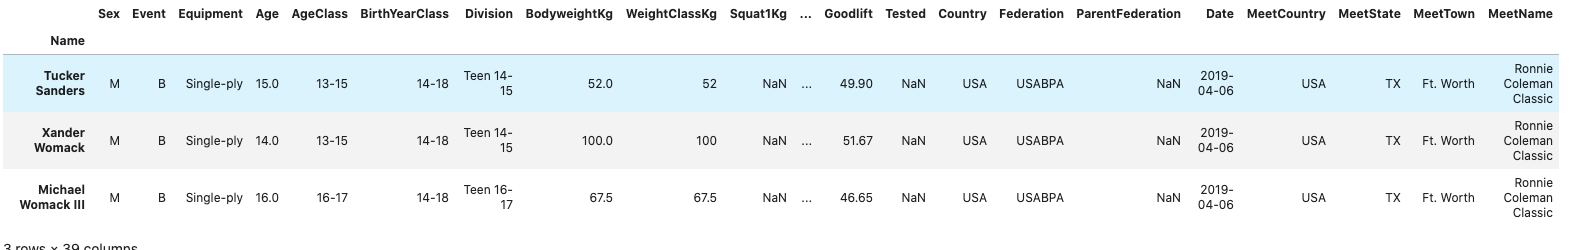
\includegraphics[width=\linewidth]{data_head.png}
\caption{データ全体}
\end{center}
\end{figure}

現状ではパワーリフティングの記録の回帰において必要のない指標も多く含まれているため、今回学習に使う指標は以下のみとする。また、今回の学習では欠損値が含まれるデータは初めから省いており、その場合におけるデータの総数は681124.である。

\begin{figure}[H]
\begin{center}
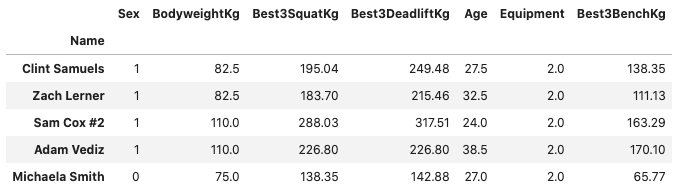
\includegraphics[width=\linewidth]{data_trimed.png}
\caption{使用するデータセット}
\end{center}
\end{figure}

それぞれの指標について簡単な説明を加えておく。一般的にパワーリフティングでは1回の試合において各競技3回まで試技を行う事が許されている。そのため、通常は試行回数を重ねるごとに記録は伸びる傾向にあるが、例えば2回目の試技では重量を持ち上げることに成功したが3回目の試技では失敗してしまった場合、3回目の試技欄には空白が入ることとなる。そのため、今回学習に用いるデータにおいてはそれぞれの試技において最高重量のみを抽出したものを使用している。また、パワーリフティングでは大会によって体にギア(図のEquipmentがそれにあたる)を着用する事が許されている場合があり、ギアを装着した場合は挙上重量が増加する傾向にある。また、それぞれの指標に対して、相関係数は下図のようになっている。

\begin{figure}[H]
\begin{center}
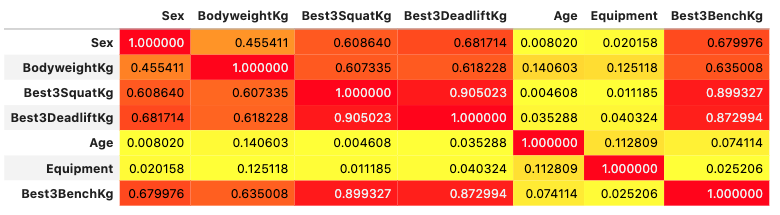
\includegraphics[width=\linewidth]{corr.png}
\caption{相関係数}
\end{center}
\end{figure}

相関係数は以下のような数式で表され、数値が1に近いほど相関があることを示している。

\begin{center}
\begin{math}
r_{xy} = \frac{\displaystyle \sum_{i = 1}^n (x_i - \overline{x})
(y_i - \overline{y})}{\sqrt{\displaystyle \sum_{i = 1}^n 
(x_i - \overline{x})^2}\sqrt{\displaystyle \sum_{i = 1}^n 
(y_i - \overline{y})^2}}
\end{math}
\end{center}

上記の表から、各競技(ベンチプレス・スクワット・デッドリフト)の重量はそれぞれ強い相関があることを示しており、年齢やギアと重量には相関が少ない事が伺える。次に、このままではデータに様々な値が存在するためにデータが扱いにくいという問題点があるため、正規化(Normalization)という手法で全てのデータを0.0から1.0の値に収まるように変換を加える必要がある。正規化は、一般的に次のように表される。

\begin{center}
\begin{math}
x_{norm(i)} = \frac{x_i - x_min }{ x_max - x_min } 
\end{math}
\end{center}

この手法でデータを扱いやすい形に変換する事ができたが、この手法は外れ値の影響を受けやすいという欠点が存在することを留意する必要がある。


\section{評価指標}

回帰分析とは、説明変数\begin{math}X\end{math}に対し目的変数\begin{math}Y\end{math}が得られる分析の事である。したがって、正解値\begin{math}T\end{math}を目的変数\begin{math}Y\end{math}がどの程度正確に予測できいるかを調べる必要がある。今回の研究では、学習モデルの評価には決定係数(\begin{math}R^2\end{math})と平均絶対誤差(MAE)の2つの指標を用いることとする。

\subsection{決定係数}

決定係数は予測値\begin{math}Y\end{math}と正解値\begin{math}T\end{math}の相関を表す。一般的に決定係数は\begin{math}R^2\end{math}で示され、以下の数式で表される。

\begin{center}
\begin{math}R^2=1-\frac{\sum_{i=1}^{n}(T_i-\hat{Y_i})^2}{\sum_{i=1}^{n}(T_i-\bar{Y_i})^2}\end{math}
\end{center}

\begin{math}R^2\end{math}は予測値\begin{math}Y\end{math}と正解値\begin{math}T\end{math}が完全に一致する場合に1となり、1に近いほど精度の高い予測が行えていることを表す。


\subsection{平均絶対誤差}

平均絶対誤差(MAE)とは代表的な誤差関数の一つであり、以下のような数式で表される。

\begin{center}
\begin{math}
MAE = \frac{\sum_{i=1}^{n}|T_i-\hat{Y_i}|}{n} 
\end{math}
\end{center}

平均絶対誤差は尤度関数と密接に結びついている。他に尤度関数と密接に関係する指標として二乗平均平方根誤差(RMSE)が挙げられるが、平均絶対誤差は二乗平均平方根誤差に比べて外れ値の影響を受けにくいという特徴がある。パワーリフティングは、一般的にはベンチプレス・スクワット・デッドリフトの3種目の重量の合計値を競うものであるが、パワーリフティングの一種に他にもシングルベンチプレスという競技が存在し、こちらはベンチプレスの重量のみで勝敗を競うものである。こちらの競技の参加者は一般にスクワットやデッドリフトの重量に対してベンチプレスの重量が大きくなりやすく、今回のデータセットには多くの外れ値が含まれているという観点から、本研究では平均絶対誤差を評価精度として用いることとする。


\section{学習手法}
\subsection{パーセプトロン}

\begin{math}w\end{math}を重みベクトル、\begin{math}b\end{math}をバイアスと呼ぶ時、入力した値が隠れ層を通さずに出力されるモデルを単純パーセプトロンと呼び、以下のように表される。

\begin{center}
\begin{math}
y = f(w^{T}x+b)
\end{math}
\end{center}

この時、予測値\begin{math}Y\end{math}と正解値\begin{math}T\end{math}の誤差が最小になるように重み\begin{math}w\end{math}とバイアス\begin{math}b\end{math}を学習の過程でパラメータを調整する事ができればニューラルネットワークの学習ができているという事になる。予測値と正解値にどれだけの誤差があるのかを示す指標を損失関数\begin{math}L\end{math}と呼び、これについては次節で詳しく解説する事とする。関数の最大・最小を考える場合には一般的にパラメータの偏微分(=勾配)を求める必要があり、その際に勾配法と呼ばれる手法が用いられる。勾配法とは、反復学習でパラメータを逐次的に更新し関数の値を徐々に減らしていく手法である。1回の学習でどれだけパラメータを更新するかを決定する指標を学習率(learning rate)\begin{math}\eta\end{math}、目的関数の\begin{math}\theta\end{math}に対する勾配をそれぞれ\begin{math}\eta_t,g_t\end{math}とおく時、勾配法は次のように表される。

\begin{center}
\begin{math}
\theta_{t+1} = \theta_t - \eta g_t
\end{math}
\end{center}

単純パーセプトロンでは1本の直線で分類できるデータにしか対応できないため、線形分離不可能な問題を分離する事はできない。入力・出力以外にニューロン(隠れ層)が繋がったモデルを多層パーセプトロンと呼び、この手法を用いることで線形分離不可能なデータも扱う事ができる事ができる。隠れ層には活性化関数と呼ばれる非線形変形を用いる関数を用いる必要があり、5.3節で詳しく解説することとする。勾配法では数値微分により勾配を算出したが、ネットワークの層が深くなった際に一般的なコンピュータの性能ではメモリの容量・計算時間が莫大になる事が知られている。その問題を解決するために取られる手法として一般的なものに、誤差逆伝播法という手法が挙げられる。先ほど紹介した勾配法が入力層から順番に計算をしていくモデルであることから「順伝播型ニューラルネットワーク」と呼ばれるのに対して、誤差逆伝播法では偏微分を出力層から入力層に向かって計算し、損失関数\begin{math}L\end{math}の誤差を用いて重みとバイアスを修正する。

% 損失関数は\begin{math}N\end{math}個のデータそれぞれで独立的に発生するものなので、次のように表される。

% \begin{center}
% \begin{math}
% L = \sum_{n=1}^{N}L_n
% \end{math}
% \end{center}


\subsection{損失関数}

ニューラルネットワークの学習において最適なパラメータを設定するためには関数の最小・最大値を考える必要がある事は前述の通りだが、その際に用いられる関数のことを一般に損失関数\begin{math}L\end{math}と呼ぶ。損失関数は予測値がどれだけ正解値から乖離しているかを表す指標であり、代表的なものに二乗和誤差や交差エントロピー誤差が挙げられる。一般に回帰問題では二乗和誤差が用いられ、分類問題では交差エントロピー誤差が用いられる。これは、二乗和誤差では正解値と予測値の乖離がそのまま誤差として表現されるのに対し、交差エントロピーでは自然対数eを底とするモデルの予測値と正解値の乗算で表されるため、予測値の誤差が強調されやすいという特徴に起因する。二乗和誤差は、以下のように表される。


\begin{center}
\begin{math}
L = \frac{1}{2} \sum_{k=1}^{n} (y_k - t_k)^{2}
\end{math}
\end{center}

前節で説明した通り、損失関数を最小にするためには勾配法という手法が使われるが、
また、回帰問題においてニューラルネットワークの出力層は恒等関数が用いられるが、恒等関数の損失関数として二乗和誤差を用いると、誤差逆



\subsection{活性化関数}

ニューロンの線形結合後に非線形変換を行う関数のことを活性化関数と呼ぶ。活性化関数に線形関数を用いない理由は、線形な変換を使うことは隠れ層を用いなくても実現できる事に起因する。代表的な活性化関数にはStep関数やSigmoid関数が挙げられ、活性化関数にSigmoid関数が用いられるモデルのことをロジスティック回帰と言う。Sigmoid関数は以下のように表される。



\begin{center}
\begin{math}
h(x) = \frac{1}{1+e^{-x}} 
\end{math}
\end{center}


また、Sigmoid関数の微分は次のように表されるため、

\begin{center}
\begin{math}
h'(x) = \frac{1}{1+e^{-x}} * (1 - \frac{1}{1+e^{-x}})
\end{math}
\end{center}

Sigmoid関数自身で微分を表すことができるという特徴を持つ。そのため、Sigmoidレイヤの逆伝播は順伝播の出力のみから導出する事が可能である。しかし、Sigmoid関数にも問題点が存在する。Sigmoid関数はS字カーブの関数であるが、Sigmoid関数の出力が0または1に近ずくにつれて、その微分の値は0に近づく。そのため、0と1に偏ったデータ分布ではニューラルネットワークの層を深くするにつれて勾配の値が小さくなるという問題点がある。また、例え層自体が深く無い場合でも、各層の次元数が多い場合などは勾配が消失しやすくなる。この問題を解決するために、活性化関数にSigmoid関数ではなく双曲線正接関数(hyperbolic tangent function)と呼ばれる関数が用いられ、以下のように数式で表される。


\begin{center}
\begin{math}
tanh(x) =  \frac{e^{x}-e^{-x}} {e^{x}+e^{-x}} 
\end{math}
\end{center}

Sigmoid関数が\begin{math}-\infty<x<+\infty\end{math}において\begin{math}0<h(x)<1\end{math}であるのに対し、\begin{math}-1<tanh(x)<1\end{math}となっている。また、双曲線正接関数の微分は以下のように表され、\begin{math}tanh'(0)=1\end{math}で最大値となるので、Sigmoid関数の導関数\begin{math}h'(x)\end{math}の最大値\begin{math}h'(0)=0.25\end{math}と比べて勾配が消失しにくいという特徴がある。

\begin{center}
\begin{math}
tanh'(x) =  \frac{4} {(e^x+e^{-x})^{2}} 
\end{math}
\end{center}

ニューラルネットワークは分類問題と回帰問題の両方に対応が可能だが、どちらの問題を用いるかによって出力層の活性化関数を変更する必要がある。分類問題において、出力層における活性化関数は確率を表す関数でなければならないので、出力の値が0から1の間に収まるSigmoid関数が用いられる。一方、回帰問題はある入力から数値の予測を行うものであるため、出力層には受け取った値に変換を加えずにそのまま出力する恒等関数(Identity function)が用いられる。


\subsection{最適化アルゴリズム}

ニューラルネットワークにおいて、最適なパラメータを求める問題を解くことを最適化問題と言う。最適なパラメータを求めるためには偏微分(=勾配)を手がかりにしたが、それには莫大な計算時間とメモリを要する事は前述の通りである。先ほど紹介した勾配法では、パラメータを更新するためにN個全てのデータを考慮する必要があった。この問題を解決するために使われる手法に、確率的勾配降下法という手法がが存在する。通常の勾配法ではN個のデータの全ての和を取ってからパラメータを更新したが、こちらの手法ではデータをランダムに1つ選んでパラメータを更新する。すなわち、通常の勾配法でパラメータを1回更新するのと同じ計算量でパラメータをN回更新する事ができる。この学習を繰り返し行うことで損失関数の値が徐々に下がっていく事が知られており、このデータ全体に対する反復回数をエポックと言う。

しかし、確率的勾配降下法は関数の形状が等方的でない限りは効率的な方法で勾配方向へ学習を進めないという問題点がある。この問題を解決するために、現在まで進んでいたパラメータを更新していた方向に進みやすくするというモーメンタムと呼ばれる手法が用いられ、次のように表される。なお、\begin{math}v\end{math}は物理でいう速度に対応している。


\begin{center}
\begin{math}
v_t := \alpha v_{t-1} - \eta  \frac{\partial L}{\partial W}
\end{math}
\end{center}

\begin{center}
\begin{math}
W_t := W_{t-1} + v_t
\end{math}
\end{center}


勾配法のもう一つの問題点として、、学習率\begin{math}\eta\end{math}が小さすぎると学習が進まず、大きすぎると学習がうまく進まない事が挙げられる。そこで、学習の過程で学習率\begin{math}\eta\end{math}を徐々に小さくすればよい。これを擬似的に再現したものが、以下のように表される。


\begin{center}
\begin{math}
h_t := h_{t-1} +  \frac{\partial L}{\partial W} \cdot \frac{\partial L}{\partial W}
\end{math}
\end{center}


\begin{center}
\begin{math}
W_t := W_{t-1} - \eta \frac{1}{\sqrt{h}} \frac{\partial L}{\partial W}
\end{math}
\end{center}

hはこれまでの勾配の値を2乗和として保持し単調増加するため、学習率が徐々に小さくなっていることが伺える。


\section{実験結果}

実際に、先述したデータセット、評価指標、そして学習手法を利用し、ベンチプレスの回帰予測の精度を確かめてみる。今回の実験ではPyhtonのバージョン3.8.6系を使用し、実行環境はDocker Hubが提供するjupyter/datascience-notebookを使用する。まずは必要なライブラリ群をインポートする。
\\


\begin{python}
import numpy as np
import matplotlib.pyplot as plt
from sklearn.model_selection import train_test_split
import pandas
from tensorflow.keras.models import Sequential
import tensorflow as tf
from tensorflow.keras.layers import Dense
from tensorflow.keras import optimizers
from keras.callbacks import EarlyStopping
from keras.layers.normalization import BatchNormalization
\end{python}


次に、使用するデータ元からデータを読み取り、カテゴリカル変数を適当なスカラー値に変換し、不要なカラムを取り除く。
\\

\begin{python}
csv = './openpowerlifting-2020-09-06.csv'
df = pandas.read_csv(csv,index_col=0,low_memory=False)
df['Sex'] = df['Sex'].map({'M': 1, 'F': 0, 'Mx': -1})
df['Equipment'] = df['Equipment'].map({'Single-ply':0, 'Raw':1, 'Wraps':2, 'Unlimited':3, 'Multi-ply':4})
data = df[['Sex','BodyweightKg', 'Best3SquatKg', 'Best3DeadliftKg','Age','Equipment', 'Best3BenchKg']].dropna(how='any')
\end{python}


\section{Conclusion}
``I always thought something was fundamentally wrong with the universe'' \citep{adams1995hitchhiker}

\bibliographystyle{plain}
\bibliography{references}
\end{document}
